% DO NOT COMPILE THIS FILE DIRECTLY!
% This is included by the other .tex files.

\begin{frame}[t,plain]
\titlepage
\end{frame}

\begin{frame}[t]{Temática}
La realización de auditorías tanto de sistemas como aplicaciones es una conducta regular en áreas informáticas o de desarrollo, de las cuales se desprenden secciones completamente dedicadas al tema, incluso haciendo uso de recompensas para individuos que encuentren e informen fallas en los sistemas pertinente. 

\begin{itemize}
\item Encapsulamiento de la Aplicación.
\item Seguridad.
\item Comprensión de Errores en el Sistema.
\end{itemize}

\bigskip
\textbf{Problemática}: Escoger una aplicación popular a auditar, realizando una búsqueda de posibles problemas y licencias asociadas a la misma app.
\bigskip

\end{frame}

\begin{frame}[t,fragile]{Qu\'e es Instagram?}
\begin{wrapfigure}{l}{0.43\textwidth} 
\vspace{2pt}
  \begin{center}
    
\includegraphics[width=0.4\textwidth]{ig}
    \label{fig:databaseUserTable}
  \end{center}
  \vspace{2pt}
\end{wrapfigure} 

Red Social que permite compartir imágenes y vídeos, aplicando efectos fotográficos del tipo : filtros, marcos, retro, vintage, entre otros, los cuales pueden ser vistos tanto en la aplicación como en otros entornos (Facebook, Twitter, Flickr, etc). 
Entre sus plataformas disponibles se encuentra:
\begin{center}
    \begin{itemize}
        \item Sistema Operativo Android.
        \item Sistema Operativo IOs.
        \item Escritorio
    \end{itemize}
\end{center}

\end{frame}

\begin{frame}[t,fragile]{Equipo de la Empresa}


\textbf{Equipo de la Empresa}
\bigskip

\begin{itemize}
    \item \textbf{Kevin Systrom (CEO, co-founder)} :  Consejero delegado o Director ejecutivo de Instagram, siendo el responsable de la visión y estrategia de la compañoa acorde a las operaciones diaria de la misma.
    \item \textbf{Mike Krieger (CTO, co-founder)} : Responsable técnico del desarrollo como la cabeza de ingeniería en Instagram, encargado de la construcción y aporte creativo del producto.
\end{itemize}
\end{frame}


\begin{frame}[t,fragile]{Desarrolladores Actuales}
\bigskip
\textbf{Desarrolladores}
\bigskip

\begin{wrapfigure}{r}{0.3\textwidth} 
\vspace{1pt}
  \begin{center}
    
\includegraphics[width=0.4\textwidth]{fbig.png}
    \label{fig:databaseUserTable}
  \end{center}
  \vspace{2pt}
\end{wrapfigure}

Actualmente los desarrolladores designados a la empresa son Facebook,  dando paso a funcionalidades similares, como lo son direct (inbox) y etiquetados de usuarios en las fotos compartidas (entre las destacadas). De ésta manera se logra la conectividad interna entre ésta (IG) y el resto de aplicaciones.

\end{frame}


\begin{frame}[t,fragile]{Licencias y Softwares Asociados}
Los software y licencias asociadas a la aplicación son los siguientes:
AFNetworking, Appirater, Boost, CocoaLumberjack, Cocoawithlove, Flick-OAuth-iOS
    ,Google Breakpad entre muchos otros
\bigskip


DE los cuales se hace una subdivisión por:

\begin{itemize}
    \item Creación de Servicios (Android y iOS)
    \item Conexión a Servidores (Android y iOS)
    \item Aplicaciones Propias de dispositivos (Android y iOS)
\end{itemize}



\end{frame}


\begin{frame}[t,fragile]{Data de Problemas Relevantes}

\textbf{Vulnerabilidad en OAuth 2013}


\begin{wrapfigure}{l}{0.43\textwidth} 
\vspace{2pt}
  \begin{center}
    
\includegraphics[width=0.4\textwidth]{oauth}
    \label{fig:databaseUserTable}
  \end{center}
  \vspace{2pt}
\end{wrapfigure} 

\bigskip

Luego de la compra de Facebook , se logra encontrar una falla de seguridad del software relacionada a la privacidad y confidencialidad de los datos, utilizando el protocolo OAuth. Dicho problema abrió paso a problemas como el acceso a la lista de amigos en Fb o filtración de imgenes.




\end{frame}

\begin{frame}[t,fragile]{Data de Problemas Relevantes}

\textbf{Cuentas Compartidas 2016}


\begin{wrapfigure}{r}{0.43\textwidth} 
\vspace{2pt}
  \begin{center}
    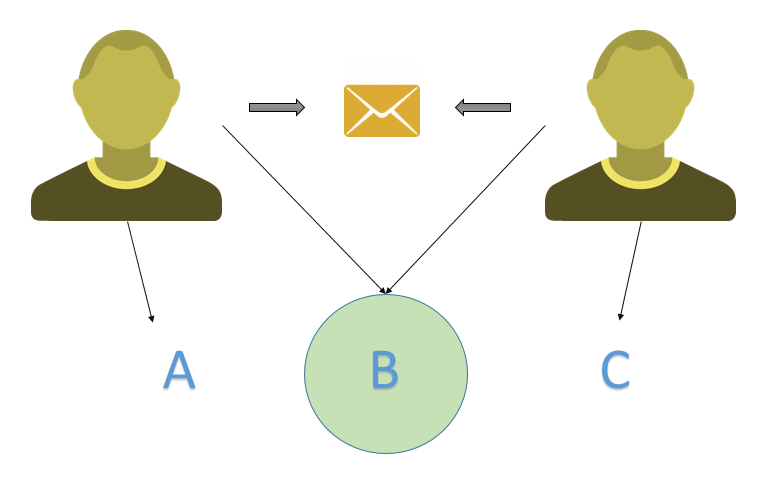
\includegraphics[width=0.5\textwidth]{compartidaig.png}
    \label{fig:databaseUserTable}
  \end{center}
  \vspace{2pt}
\end{wrapfigure} 

\bigskip

Consiste en la compartición de cuentas por parte de un Sujeto 1 v's un Sujeto 2, donde ambos ya sea por motivos de asociación u otros comparten una cuenta en común B, dando paso a la notificación de cuentas fuera de su alcance. Lo que implica una filtración de información fuera del consentimiento de cada sujeto.

\end{frame}


\begin{frame}[t,fragile]{Data de Problemas Relevantes}

\textbf{Hackeo de Cuentas 2017}


\begin{wrapfigure}{l}{0.43\textwidth} 
\vspace{2pt}
  \begin{center}
    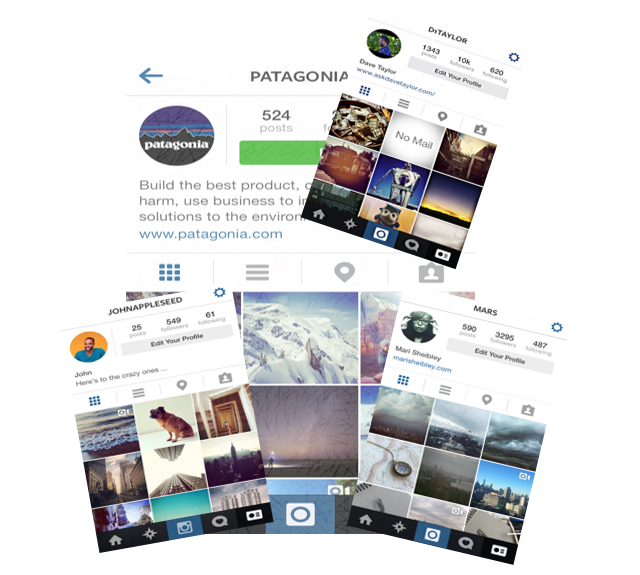
\includegraphics[width=0.45\textwidth]{accounts.png}
    \label{fig:databaseUserTable}
  \end{center}
  \vspace{2pt}
\end{wrapfigure} 

\bigskip

Hackeo masivo de cuentas, comprometiendo la seguridad de las cuentas en redes sociales. Llegando a circular datos de acceso a los perfiles a \$10 dolares cada cuenta. La información fue almacenada en la base de datos \textbf{Doxagram} en donde se realizó la venta.



\end{frame}

\begin{frame}[t,fragile]{Descarga de Aplicación}

\textbf{Obtención de Apk}


\begin{figure}[!h]
    \centering
    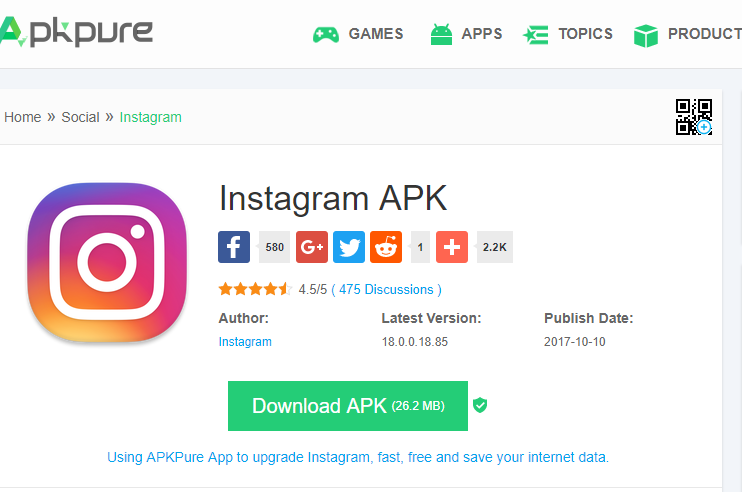
\includegraphics[scale=0.4]{apkpure.png}
    \label{fig:my_label}
\end{figure}

\end{frame}

\begin{frame}[t,fragile]{Decompilación}

\textbf{Obtención de Archivos}


\begin{wrapfigure}{r}{0.43\textwidth} 
\vspace{2pt}
  \begin{center}
    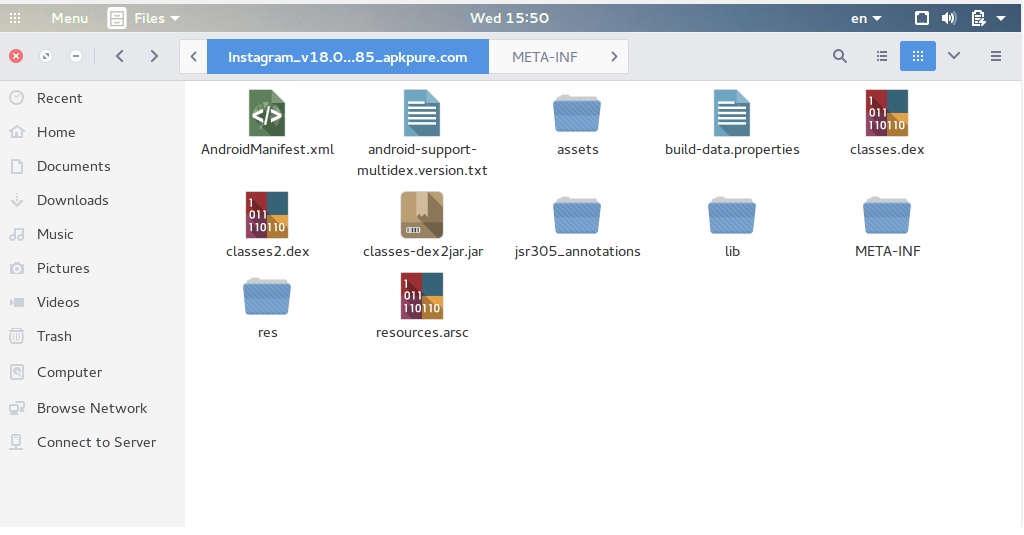
\includegraphics[width=0.45\textwidth]{decompiladaapk.png}
    \label{fig:databaseUserTable}
  \end{center}
  \vspace{2pt}
\end{wrapfigure} 

\bigskip

Tras descargar el apk de instagram se utiliza la siguiente metodología:

\begin{itemize}
    \item Convertir archivo a .ZIP, para obtener archivos.
    \item Obtención de XML, classes.dex, lib y Meta-inf.
\end{itemize}


\end{frame}




\begin{frame}[t,fragile]{Decompilación}

\textbf{META-INF}


\begin{wrapfigure}{r}{0.43\textwidth} 
\vspace{2pt}
  \begin{center}
    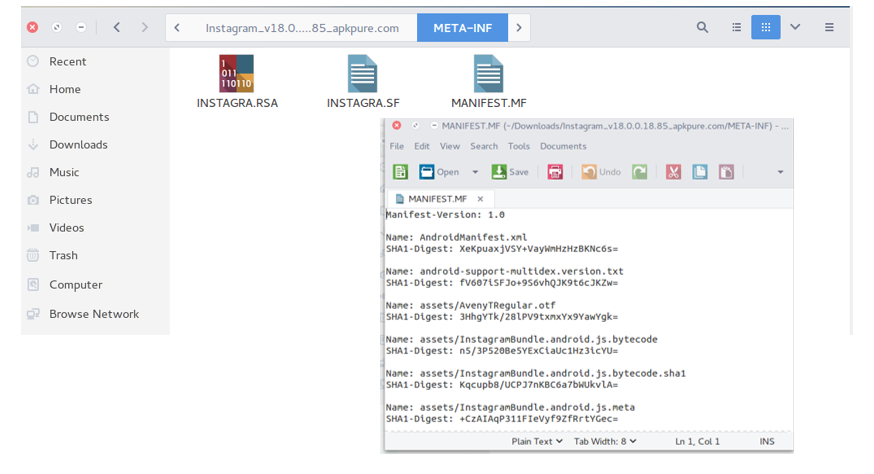
\includegraphics[width=0.45\textwidth]{meta-inf2.png}
    \label{fig:databaseUserTable}
  \end{center}
  \vspace{2pt}
\end{wrapfigure} 

\bigskip

En ésta carpeta es posible encontrar los métodos utilizados en la aplicación para la realización de encriptación y seguridad propiamente tal de los archivos dentro del desarrollo. Destacando entonces herramientas como:

\begin{itemize}
    \item RSA (cifrado)
    \item SHA1 (hashing)
\end{itemize}


\end{frame}




\begin{frame}[t,fragile]{Decompilación}

\textbf{Uso de Apktool}

\begin{wrapfigure}{r}{0.43\textwidth} 
\vspace{2pt}
  \begin{center}
    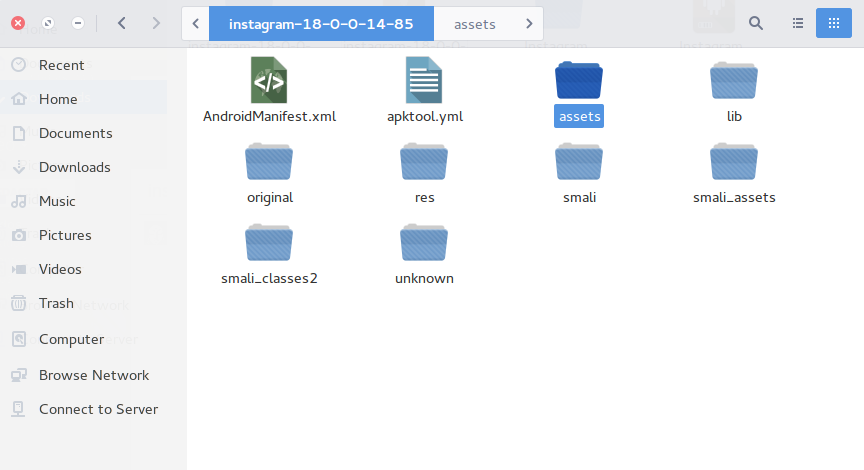
\includegraphics[width=0.45\textwidth]{apktool.png}
    \label{fig:databaseUserTable}
  \end{center}
  \vspace{2pt}
\end{wrapfigure} 

\bigskip

Uso de herramienta \textbf{apktool} 
\begin{center}
    apktool d Instagram.apk
\end{center}
 \\
 
 se obtendrá archivos correspondientes a la aplicación además de los layouts, res y clasess especificas del mismo.

\end{frame}

\begin{frame}[t,fragile]{Decompilación}

\textbf{Obtención de XML}

\begin{wrapfigure}{r}{0.43\textwidth} 
\vspace{2pt}
  \begin{center}
    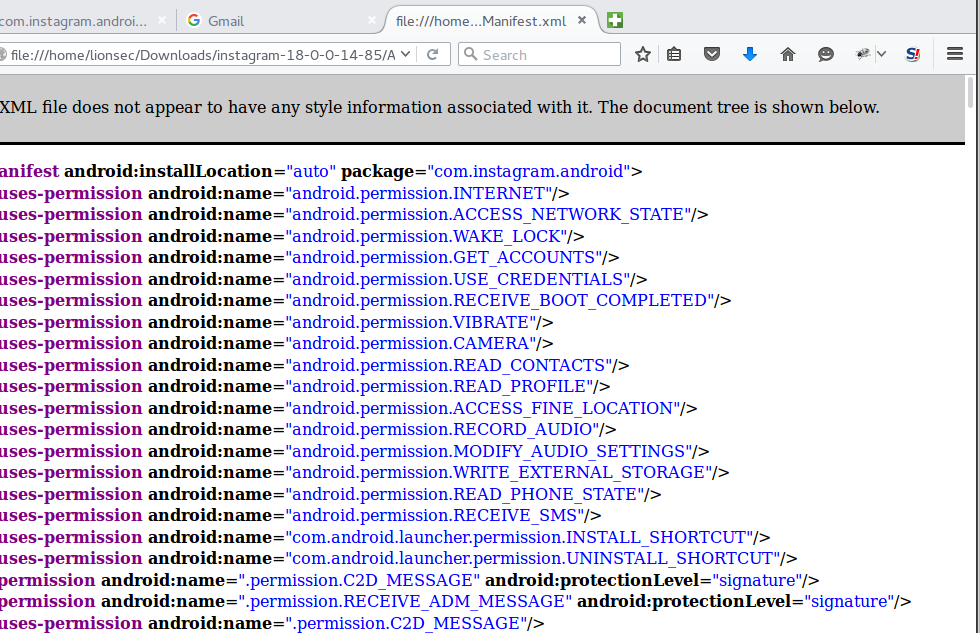
\includegraphics[width=0.45\textwidth]{xml.png}
    \label{fig:databaseUserTable}
  \end{center}
  \vspace{2pt}
\end{wrapfigure} 

\bigskip

 Por medio de la herrramienta \textbf{apktool} y utilizando consola. se aplica comando
\begin{center}
    apktool d Instagram.apk
\end{center}
 \\
 
 se obtendrá los xml y archivos correspondientes a la aplicación.

\end{frame}

\begin{frame}[t,fragile]{Decompilación}

\textbf{Obtención de Java}

\begin{wrapfigure}{r}{0.43\textwidth} 
\vspace{2pt}
  \begin{center}
    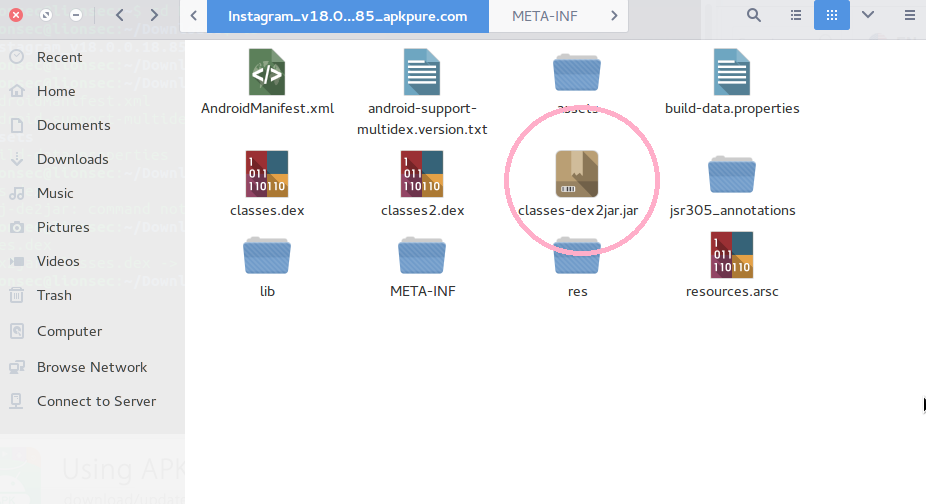
\includegraphics[width=0.45\textwidth]{jarclases.png}
    \label{fig:databaseUserTable}
  \end{center}
  \vspace{2pt}
\end{wrapfigure} 

\bigskip

 Por medio de la herramienta \textbf{dex2jar} y utilizando consola. se aplica comando
\begin{center}
    d2j-dex2jar classes.dex
\end{center}
 \\
 
 se utiliza el dex (Dalvik Executable) para obtener el comprimido del archivo APK. Lo que puede ser visto con un java decompiler, accediendo entonces a el archivo.

\end{frame}


\begin{frame}[t,fragile]{Decompilación}

\textbf{Ver Archivos React}

\begin{wrapfigure}{r}{0.43\textwidth} 
\vspace{2pt}
  \begin{center}
    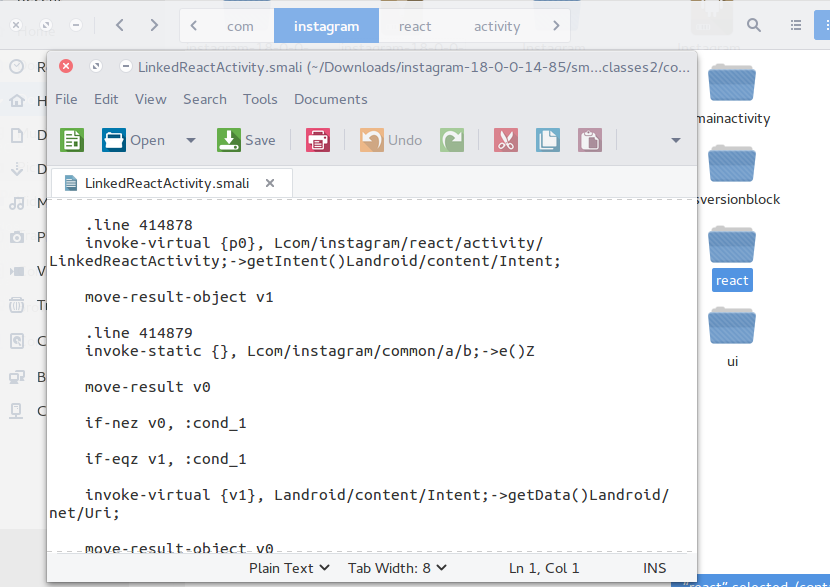
\includegraphics[width=0.45\textwidth]{react.png}
    \label{fig:databaseUserTable}
  \end{center}
  \vspace{2pt}
\end{wrapfigure} 

\bigskip

 Se encuentran los archivos de react correspondiente las actividades, delegados o bien los archivos \textbf{.smali} correspondientes al assembly de lenguaje Java.

\end{frame}


\begin{frame}[t,fragile]{Decompilación}

\textbf{Hosts}

\begin{wrapfigure}{r}{0.43\textwidth} 
\vspace{2pt}
  \begin{center}
    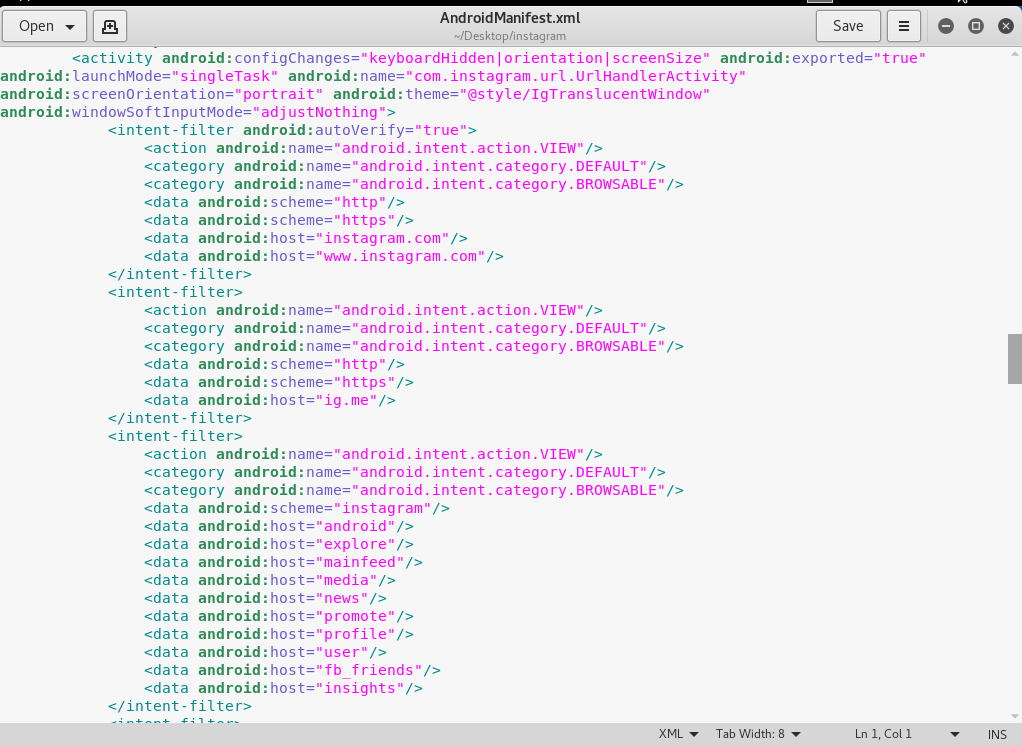
\includegraphics[width=0.45\textwidth]{xmlhost.png}
    \label{fig:databaseUserTable}
  \end{center}
  \vspace{2pt}
\end{wrapfigure} 

\bigskip

En la siguiente figura se logra apreciar el Host principal correspondiente a la aplicación, dando a entender que :

\begin{center}
    www.instagram.com    
\end{center}
será la url, host del resto de actividades.



\end{frame}

\begin{frame}[t,fragile]{Host a Probar}

\textbf{Hosts Encontrados en AndroidManifest.xml}

\begin{wrapfigure}{r}{0.43\textwidth} 
\vspace{2pt}
  \begin{center}
    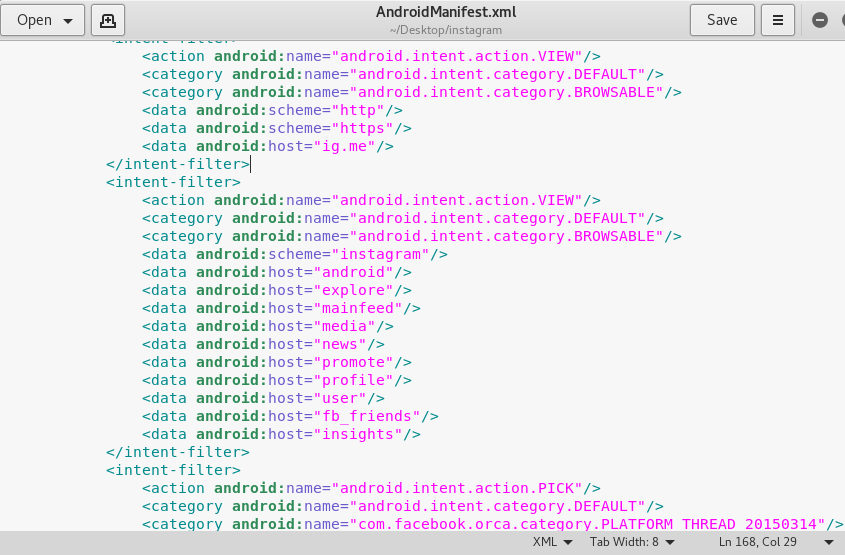
\includegraphics[width=0.45\textwidth]{xmlhostbrowser.png}
    \label{fig:databaseUserTable}
  \end{center}
  \vspace{2pt}
\end{wrapfigure} 

\bigskip

Una vez conocida la url, se procede por medio de sqlmap a analizar el siguiente listado de host (Browsers) respectivos a la api:


\begin{itemize}
\item android
\item explore
\item mainfeed
\item media
\item news
\item entre otros.
\end{itemize}

\end{frame}

\begin{frame}[t,fragile]{Herramientas}

\textbf{Uso de SQLMAP}

\begin{wrapfigure}{r}{0.43\textwidth} 
\vspace{2pt}
  \begin{center}
    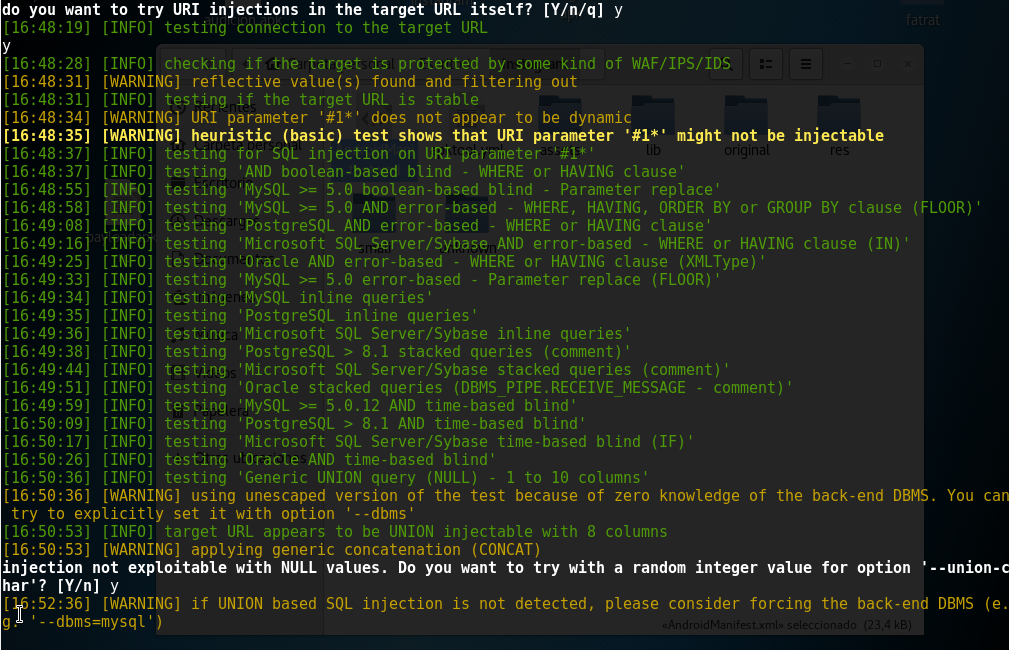
\includegraphics[width=0.45\textwidth]{testsqlmap.png}
    \label{fig:databaseUserTable}
  \end{center}
  \vspace{2pt}
\end{wrapfigure} 

\bigskip

 Tras utilizar el comando:
 
 \begin{center}
     sqlmap -u www.instagram.com/ Host Browsers 
 \end{center}
 
 Realizando inyecciones dentro de la aplicación, de tal manera que se busquen fugas o posibles consultas. 

\end{frame}


\begin{frame}[t,fragile]{Herramientas}

\textbf{Uso de SQLMAP}

\begin{wrapfigure}{r}{0.43\textwidth} 
\vspace{2pt}
  \begin{center}
    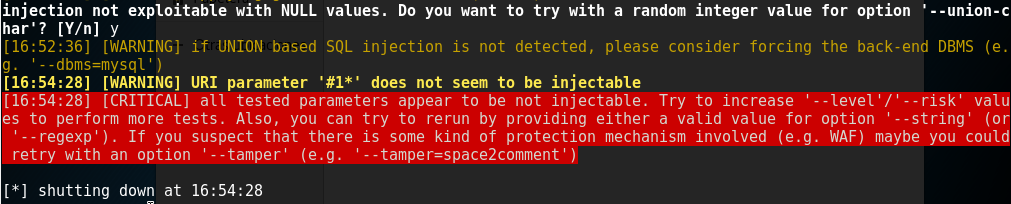
\includegraphics[width=0.45\textwidth]{errortest.png}
    \label{fig:databaseUserTable}
  \end{center}
  \vspace{2pt}
\end{wrapfigure} 

\bigskip

 Encontrando el siguiente error, lo que implica que no se logró hacer ninguna inyección exitosa dentro de la aplicación.

\end{frame}

\begin{frame}[t,fragile]{Herramientas}

\textbf{Uso de NMAP}

\begin{wrapfigure}{r}{0.43\textwidth} 
\vspace{2pt}
  \begin{center}
    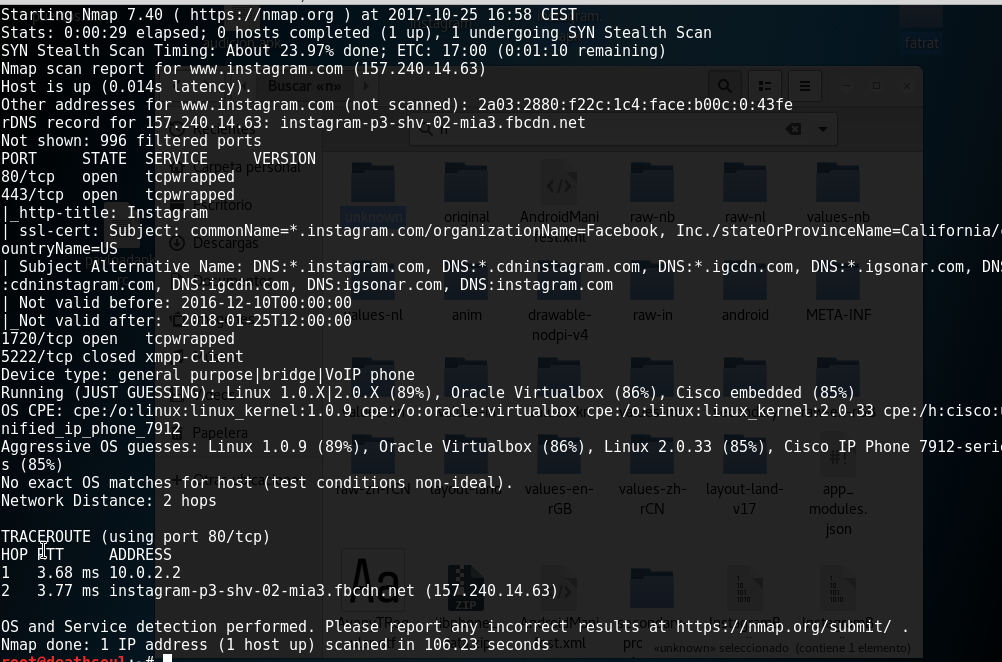
\includegraphics[width=0.45\textwidth]{nmap.png}
    \label{fig:databaseUserTable}
  \end{center}
  \vspace{2pt}
\end{wrapfigure} 

\bigskip

 Tras utilizar el comando:
 
 \begin{center}
     nmap -O www.instagram.com 
 \end{center}
 
Obteniendo los puertos abiertos dentro de la aplicación:

\begin{itemize}
    \item Puerto 80/tcp
    \item Puerto 443/tcp
\end{itemize}

\end{frame}

\begin{frame}[t,fragile]{Herramientas}

\textbf{Uso de Wireshark}

\begin{wrapfigure}{r}{0.43\textwidth} 
\vspace{2pt}
  \begin{center}
    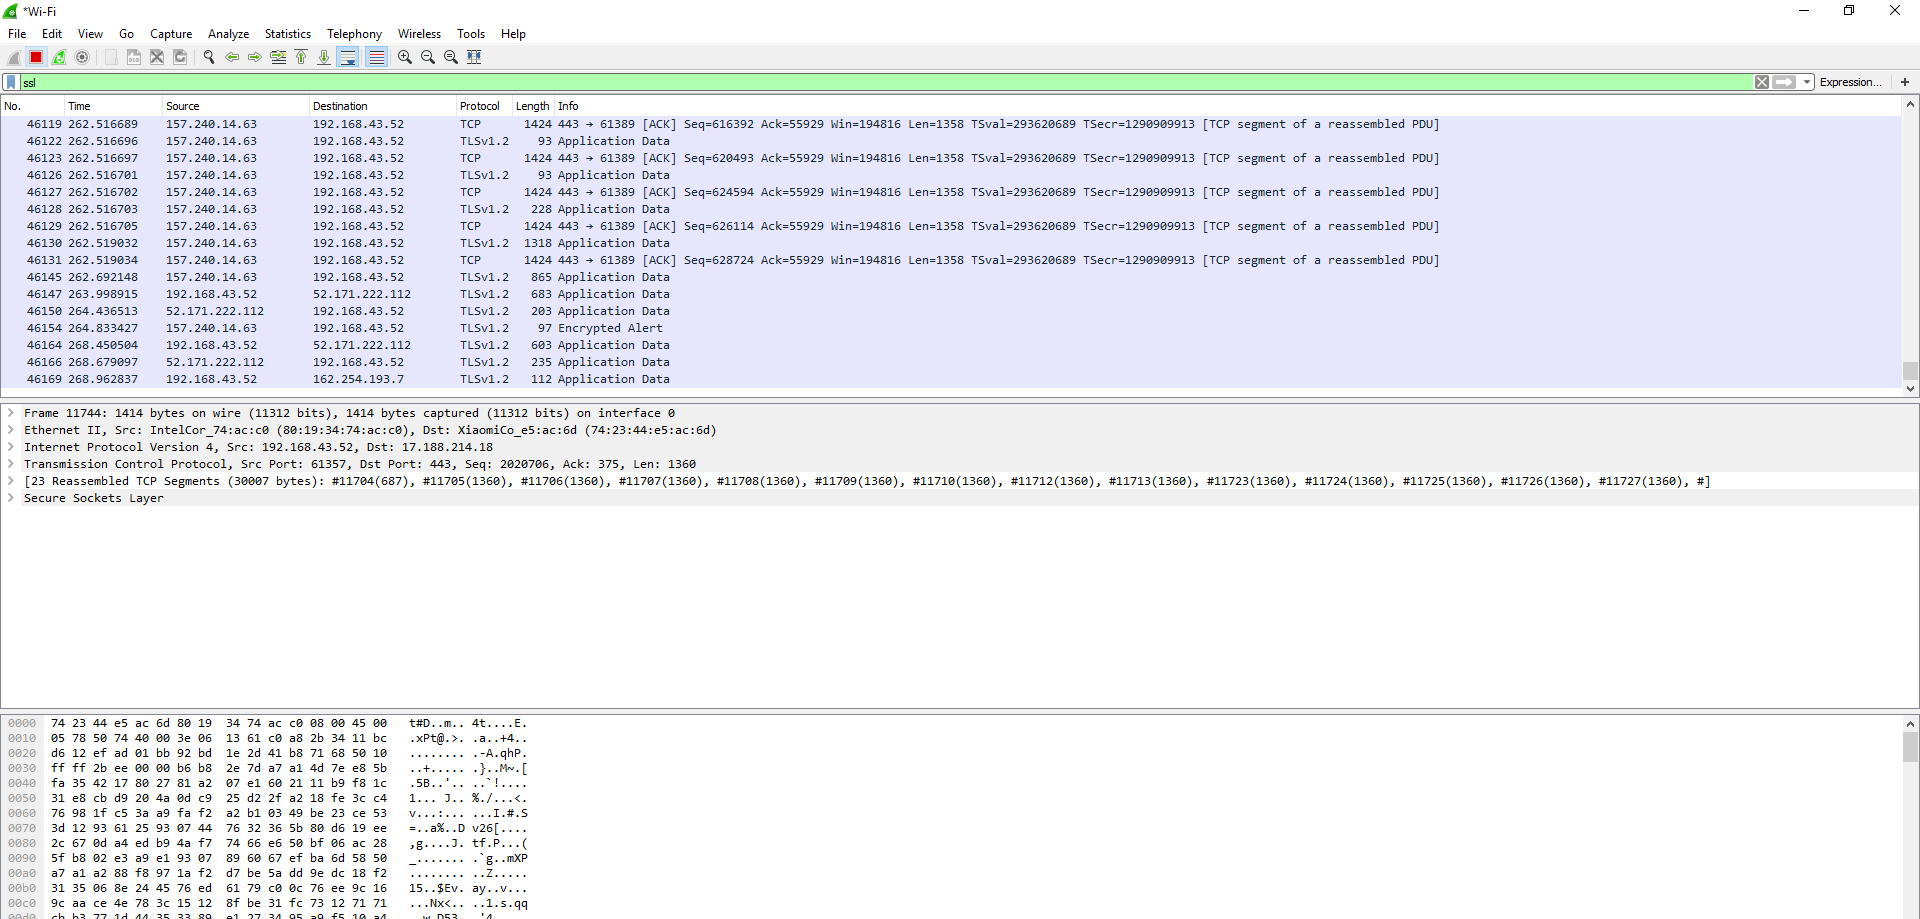
\includegraphics[width=0.45\textwidth]{wireshark.png}
    \label{fig:databaseUserTable}
  \end{center}
  \vspace{2pt}
\end{wrapfigure} 

\bigskip

Mediante el uso de wireshark, se realizan análisis de los paquetes captados en conjunto con la aplicación, de las cuales no se logra encontrar paquetes expuestos. 

\end{frame}


\begin{frame}[t,fragile]{Keylogs}

\textbf{Creación de PATH}

\begin{wrapfigure}{r}{0.43\textwidth} 
\vspace{2pt}
  \begin{center}
    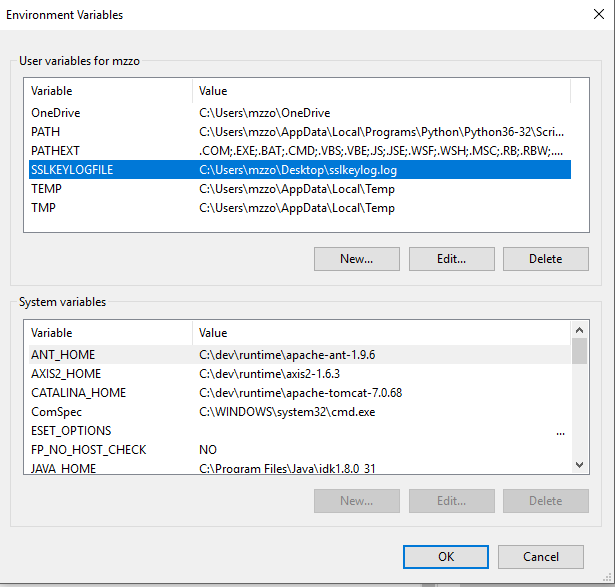
\includegraphics[width=0.45\textwidth]{sslpath.png}
    \label{fig:databaseUserTable}
  \end{center}
  \vspace{2pt}
\end{wrapfigure} 

\bigskip

Es necesario generar un nuevo PATH en las variables ambiente, declarando la dirección a apuntar y el archivo a generar, el cual será:

\begin{center}
   \textbf{sslkeylog.log}
\end{center}


\end{frame}



\begin{frame}[t,fragile]{Herramientas}

\textbf{El archivo obtenido}

\begin{wrapfigure}{r}{0.43\textwidth} 
\vspace{2pt}
  \begin{center}
    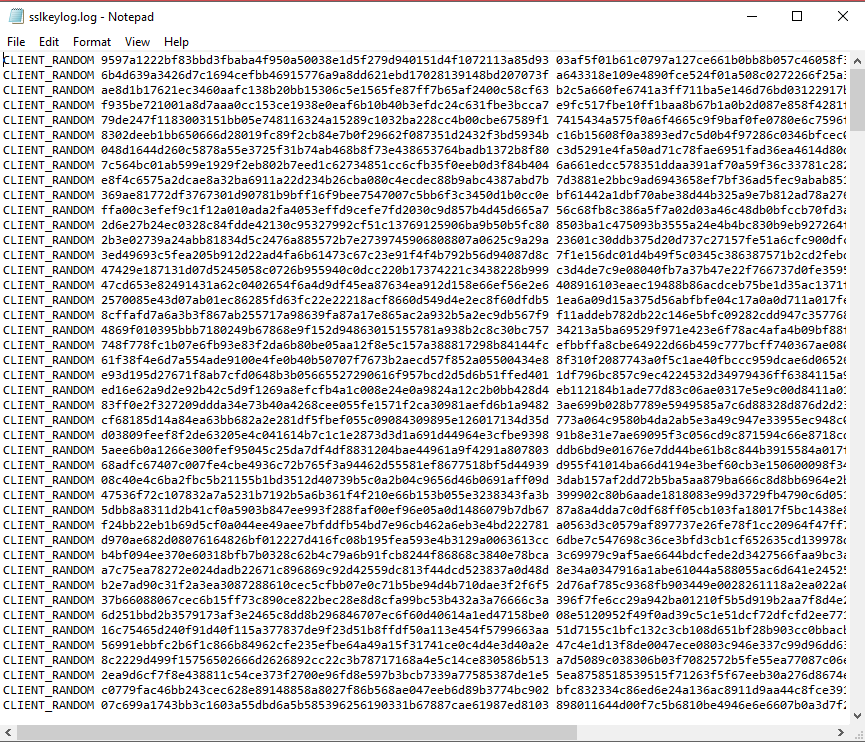
\includegraphics[width=0.45\textwidth]{ssllog.png}
    \label{fig:databaseUserTable}
  \end{center}
  \vspace{2pt}
\end{wrapfigure} 

\bigskip

Se aprecian los datos obtenidos en el archivo \textbf{sslkeylog.log}, donde se declara el cliente, llave y rsa.

\begin{center}
   
\end{center}

\end{frame}

\begin{frame}[t,fragile]{Herramientas}

\textbf{WireShark Implementación de Certificados}

\begin{wrapfigure}{r}{0.43\textwidth} 
\vspace{2pt}
  \begin{center}
    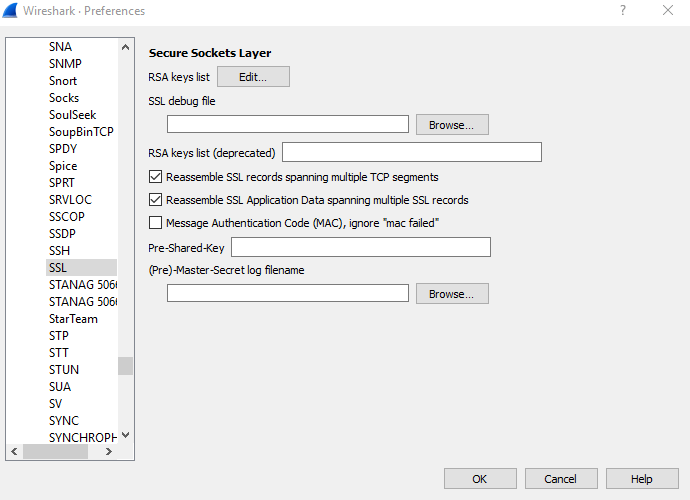
\includegraphics[width=0.45\textwidth]{wiressl.png}
    \label{fig:databaseUserTable}
  \end{center}
  \vspace{2pt}
\end{wrapfigure} 

\bigskip

Ya en previa emisión de internet por parte del computador, es necesario proveer los certificados generados, contal de ver la respuesta dentro de la aplicación.

\begin{center}
   
\end{center}

\end{frame}

\begin{frame}[t,fragile]{Herramientas}

\textbf{Búsqueda de Carpeta con Certificados }

\begin{wrapfigure}{r}{0.43\textwidth} 
\vspace{2pt}
  \begin{center}
    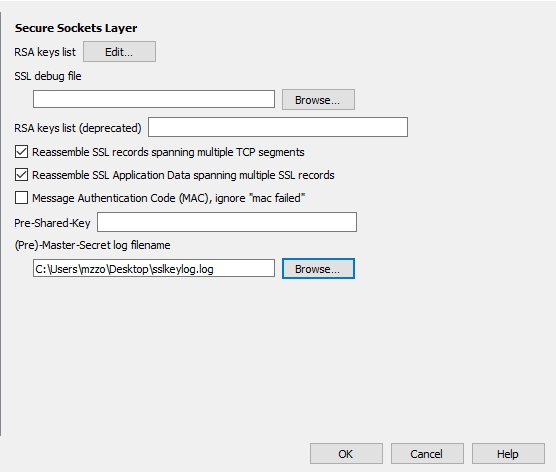
\includegraphics[width=0.45\textwidth]{archivossllog.png}
    \label{fig:databaseUserTable}
  \end{center}
  \vspace{2pt}
\end{wrapfigure} 

\bigskip

Es necesario proveer la ruta especifica en donde se encuentra el archivo generado por el PATH, de tal manera que trabajen como decifradores de las request generadas al hacer man-in-the-middle.


\end{frame}



\begin{frame}[t,fragile]{Herramientas}

\textbf{Uso de Wireshark}

\begin{wrapfigure}{r}{0.43\textwidth} 
\vspace{2pt}
  \begin{center}
    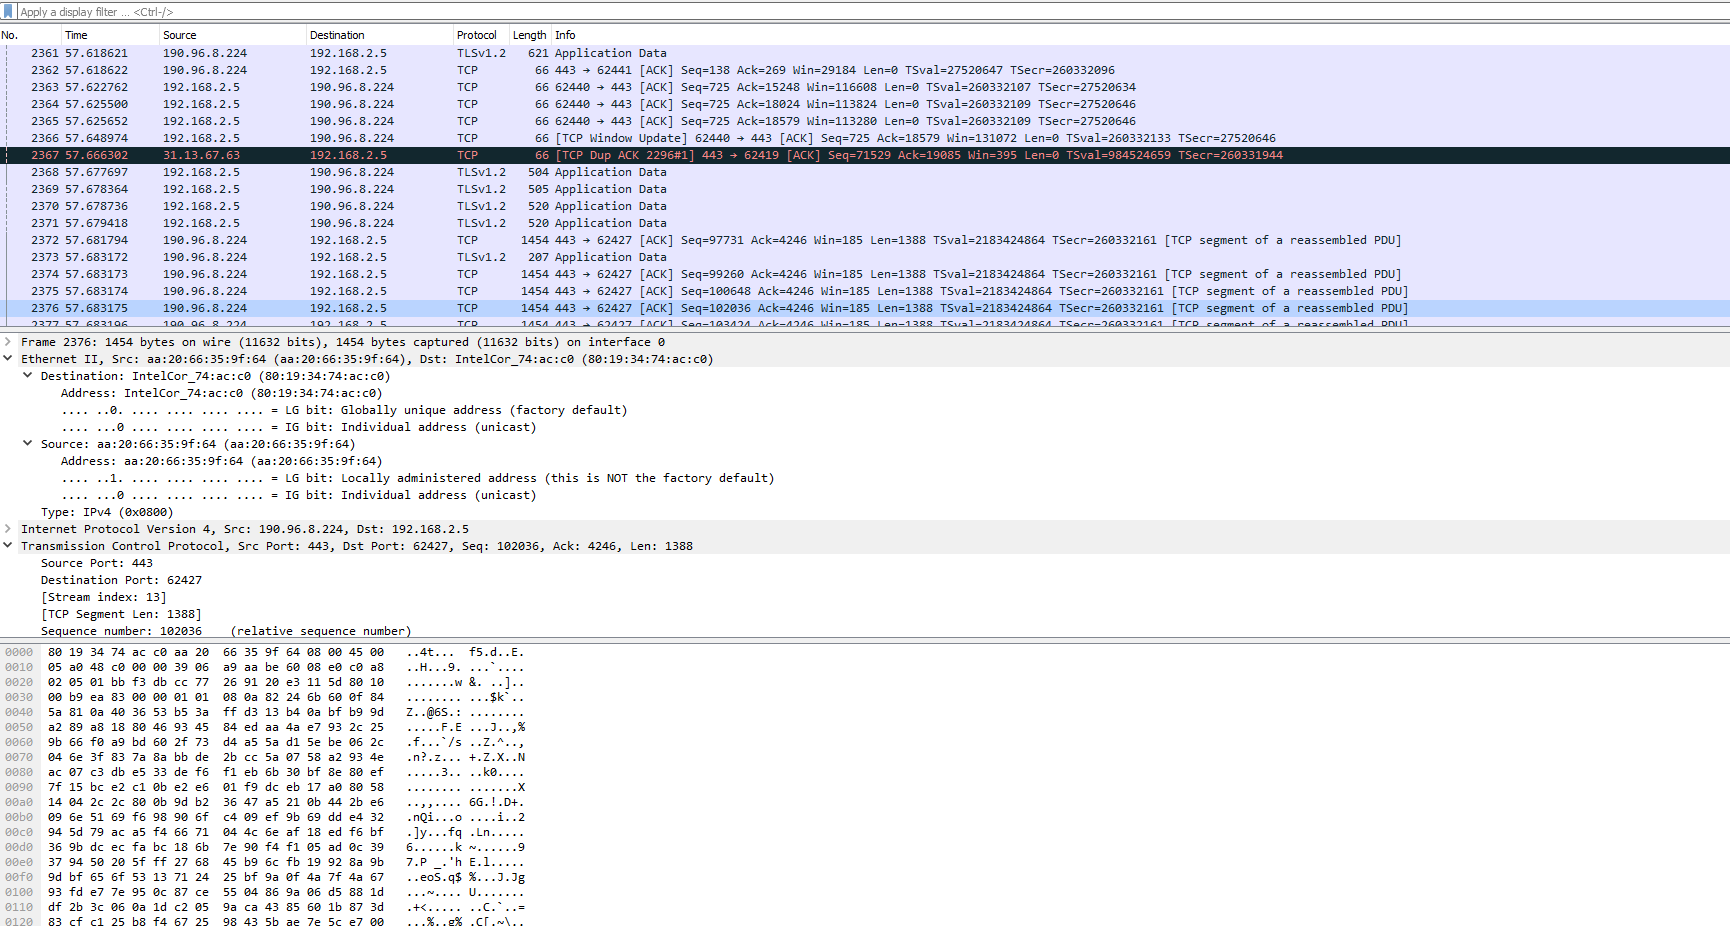
\includegraphics[width=0.45\textwidth]{paqueteswiressl.png}
    \label{fig:databaseUserTable}
  \end{center}
  \vspace{2pt}
\end{wrapfigure} 

\bigskip

Se adjunta las imagen correspondiente a los paquetes recibidos dentro de la aplicación haciendo uso del celular como emisor de paquetes, de entre los cuales se logra apreciar ciertos paquetes.


\end{frame}


\begin{frame}[t,fragile]{Herramientas}

\textbf{Uso de Wireshark}

\begin{wrapfigure}{r}{0.43\textwidth} 
\vspace{2pt}
  \begin{center}
    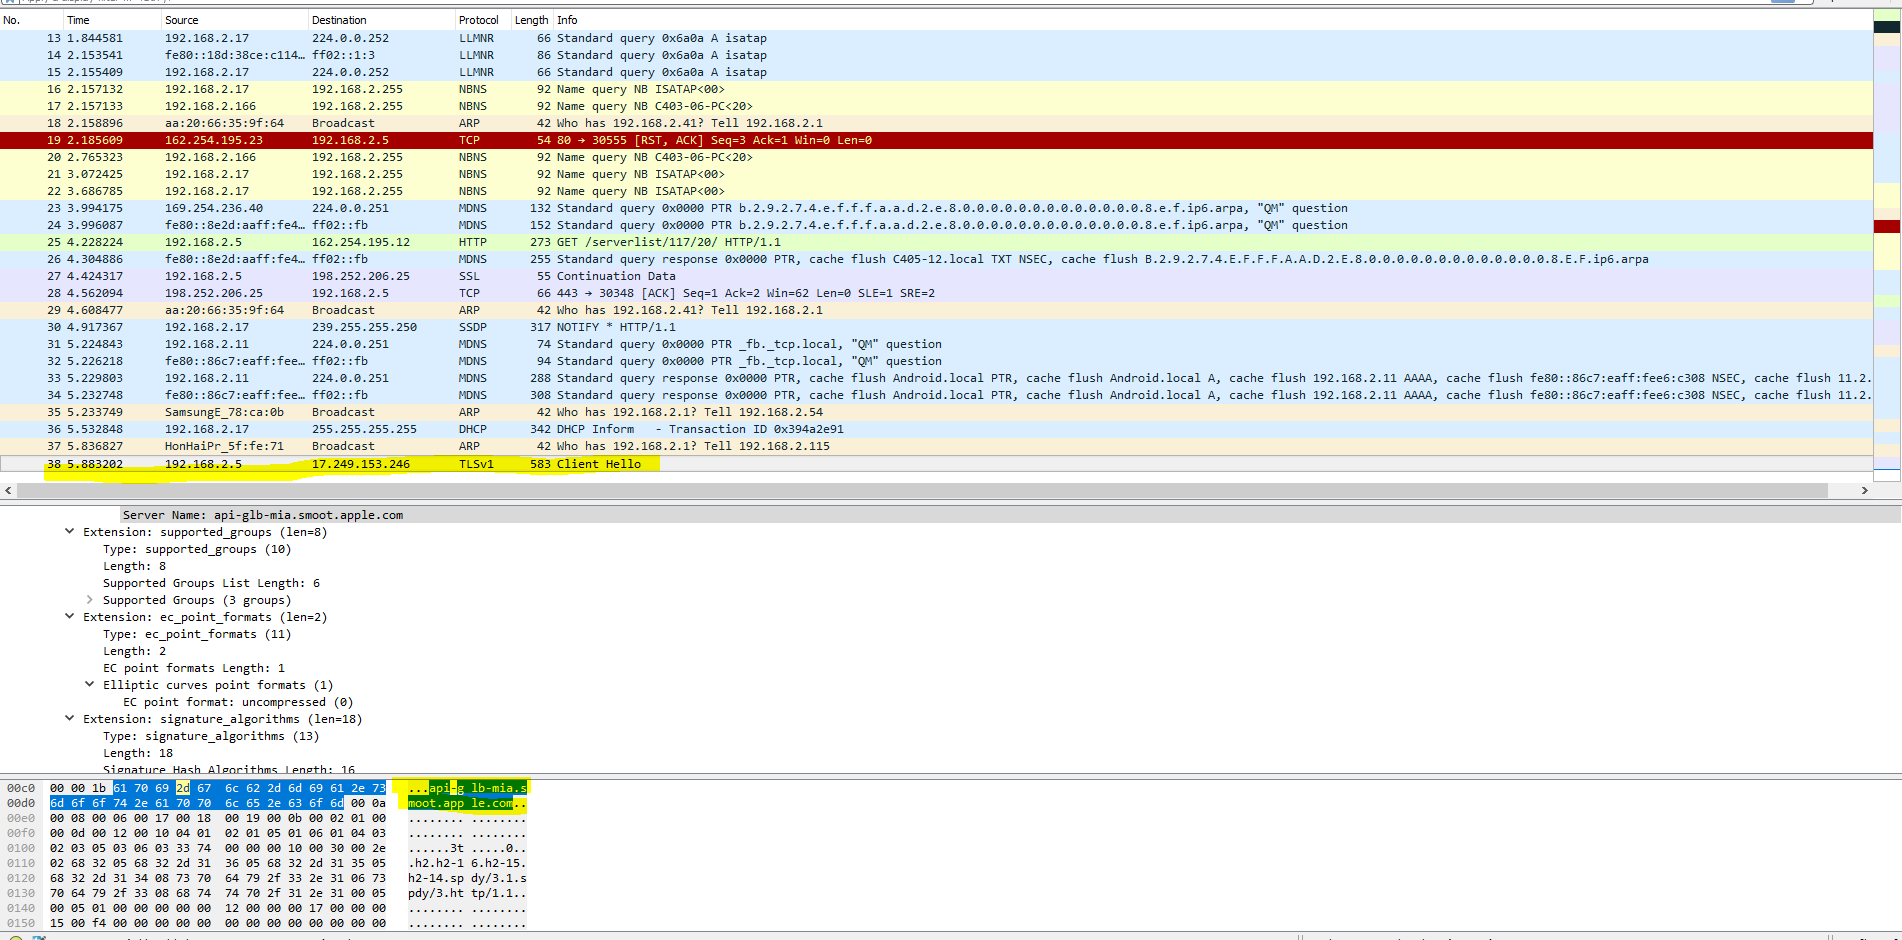
\includegraphics[width=0.45\textwidth]{paquetelectura.png}
    \label{fig:databaseUserTable}
  \end{center}
  \vspace{2pt}
\end{wrapfigure} 

\bigskip

Es posible apreciar lectura de los paquetes, entregando pauetes del tipo TCP y CLIENT HELLO, de la cuál se adjunta una recepción del paquete mayormente ilegible, pero aún así, no se encuentra información consistente y tangible de las respuestas. Lo que implica que no es posible captar la información de los usuarios o bien sentencias explotables.


\end{frame}

\begin{frame}[t,fragile]{Obtención de IP}

\textbf{Utilizar ping en CMD}

\begin{wrapfigure}{r}{0.43\textwidth} 
\vspace{2pt}
  \begin{center}
    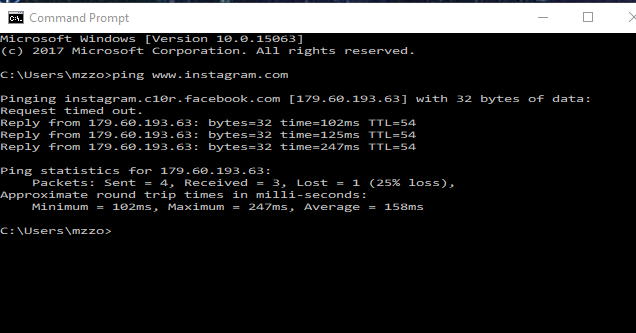
\includegraphics[width=0.48\textwidth]{pinginstagram.png}
    \label{fig:databaseUserTable}
  \end{center}
  \vspace{2pt}
\end{wrapfigure} 

\bigskip

Por medio de la consola predispuesta por windows y el uso de la url \emph{www.instagram.com}, se realiza un diagnostico de la determinada red, con el fin de conseguir su respectiva IP. 
Entonces se utiliza:

\begin{center}
   \textbf{ping www.instagram.com}
\end{center}

se obtiene

\begin{center}
   \textbf{179.60.193.63}
\end{center}





\end{frame}



\begin{frame}[t,fragile]{Herramientas}

\textbf{Metasploit}

\begin{wrapfigure}{r}{0.43\textwidth} 
\vspace{2pt}
  \begin{center}
    
\includegraphics[width=0.5\textwidth]{meta.jpg}
    \label{fig:databaseUserTable}
  \end{center}
  \vspace{2pt}
\end{wrapfigure} 

\bigskip

 Herramienta  utilizada para desarrollar y ejecutar exploits contra una máquina remota, generando scripts de utilidad, declarando ejercicios como DoS u otros, de tal manera de generar pruebas dentro de la IP obtenida.


\end{frame}

\begin{frame}[t,fragile]{Herramientas}

\textbf{Lineas de Comando}

\begin{wrapfigure}{r}{0.43\textwidth} 
\vspace{2pt}
  \begin{center}
    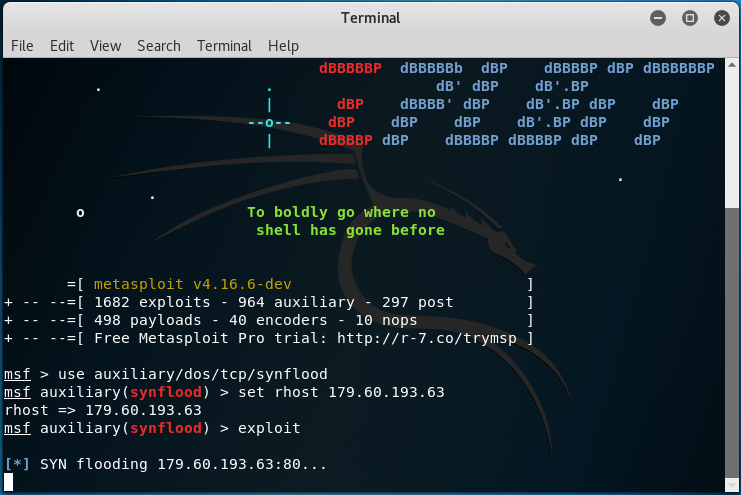
\includegraphics[width=0.45\textwidth]{sploit.png}
    \label{fig:databaseUserTable}
  \end{center}
  \vspace{2pt}
\end{wrapfigure} 

\bigskip

Se dispone a utilizar el siguiente comando \textbf{use auxiliary/dos/tcp/synflood}, donde se provee \textbf{auxiliary}, el cual permite la obtención de información sobr el objetivo, con tal de determinar las posibles vulnerabilidades. Además de proveer el protocolo \textbf{tcp} y  el tipo de ataque a realizar, el cual para este caso corresponde a \textbf{dos} y \textbf{synflood} 

\end{frame}

\begin{frame}[t,fragile]{Herramientas}

\textbf{Lineas de Comando}

\bigskip

Finalmente se setea el \textbf{rhost} ligado a la IP \textbf{179.60.193.63} para finalmente ejecutar el exploit generado.

\begin{figure}[!h]
    \centering
    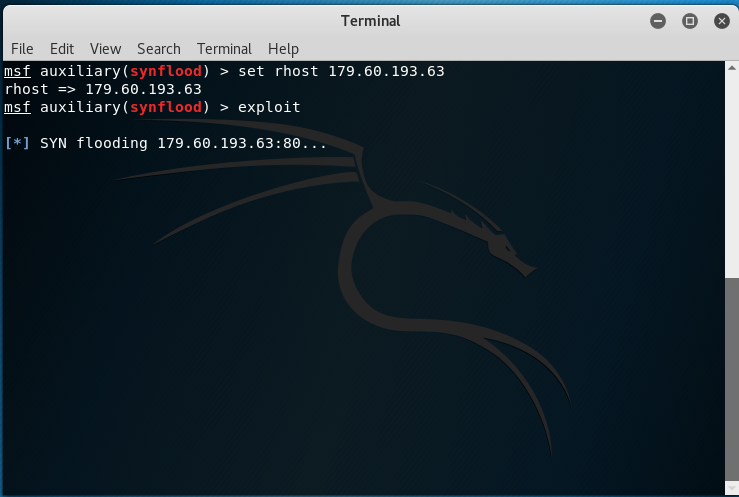
\includegraphics[scale=0.35]{metaesploit.png}
    \label{fig:my_label}
    \end{figure}

\end{frame}



\begin{frame}[t,fragile]{Herramientas}

\textbf{Wireshark}

\bigskip

A continuación se da a conocer una vista del envio de paquetes al realizar el exploit mencionado anteriormente.

\begin{figure}[!h]
    \centering
    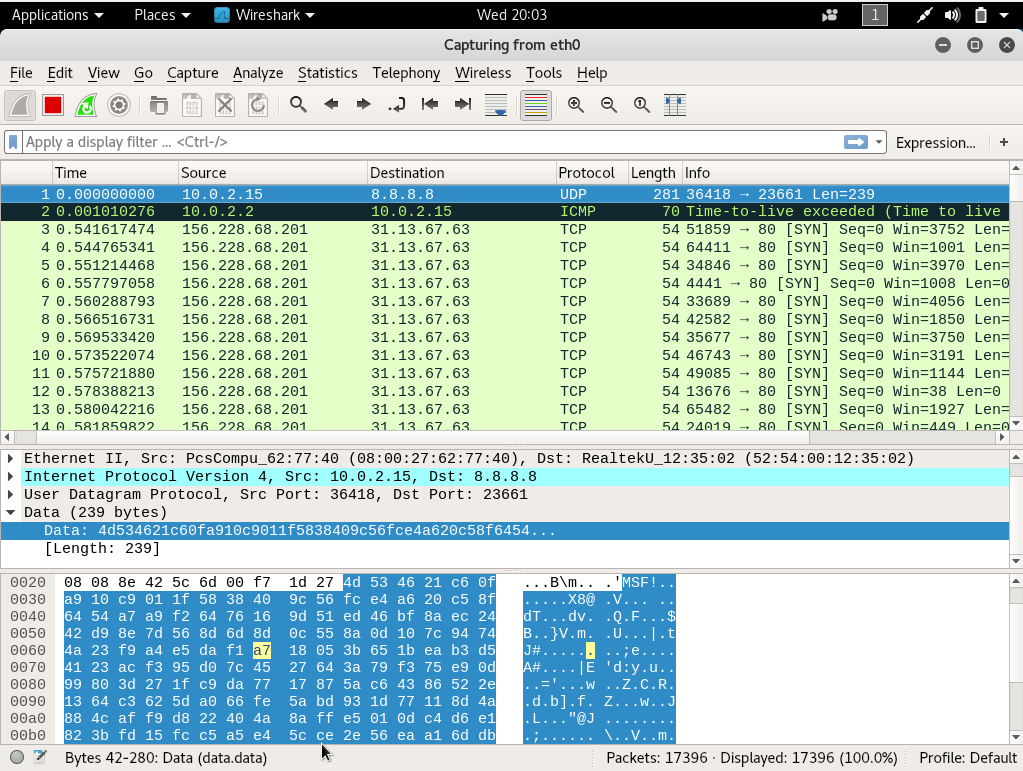
\includegraphics[scale=0.25]{wireshark5.png}
    \label{fig:my_label}
    \end{figure}

\end{frame}


\begin{frame}[t,fragile]{Conclusión}

\textbf{Imposibruh}



\begin{figure}[!h]
    \centering
    
\includegraphics[scale=0.45]{instagram-logo.png}
    \label{fig:my_label}
    \end{figure}

\end{frame}

